\documentclass[11pt,a4paper,oneside]{article}
\usepackage[UTF8,adobefonts]{ctex}

\usepackage{wrapfig}
\usepackage{indentfirst}
\usepackage{amsmath}
\usepackage{float}
\usepackage{ulem}

\usepackage[top=1in,bottom=1in,left=1.25in,right=1.25in]{geometry}

\usepackage{color}
\usepackage{xcolor}

\usepackage{multirow}

\begin{document}

\begin{figure}[H]
 \centering
  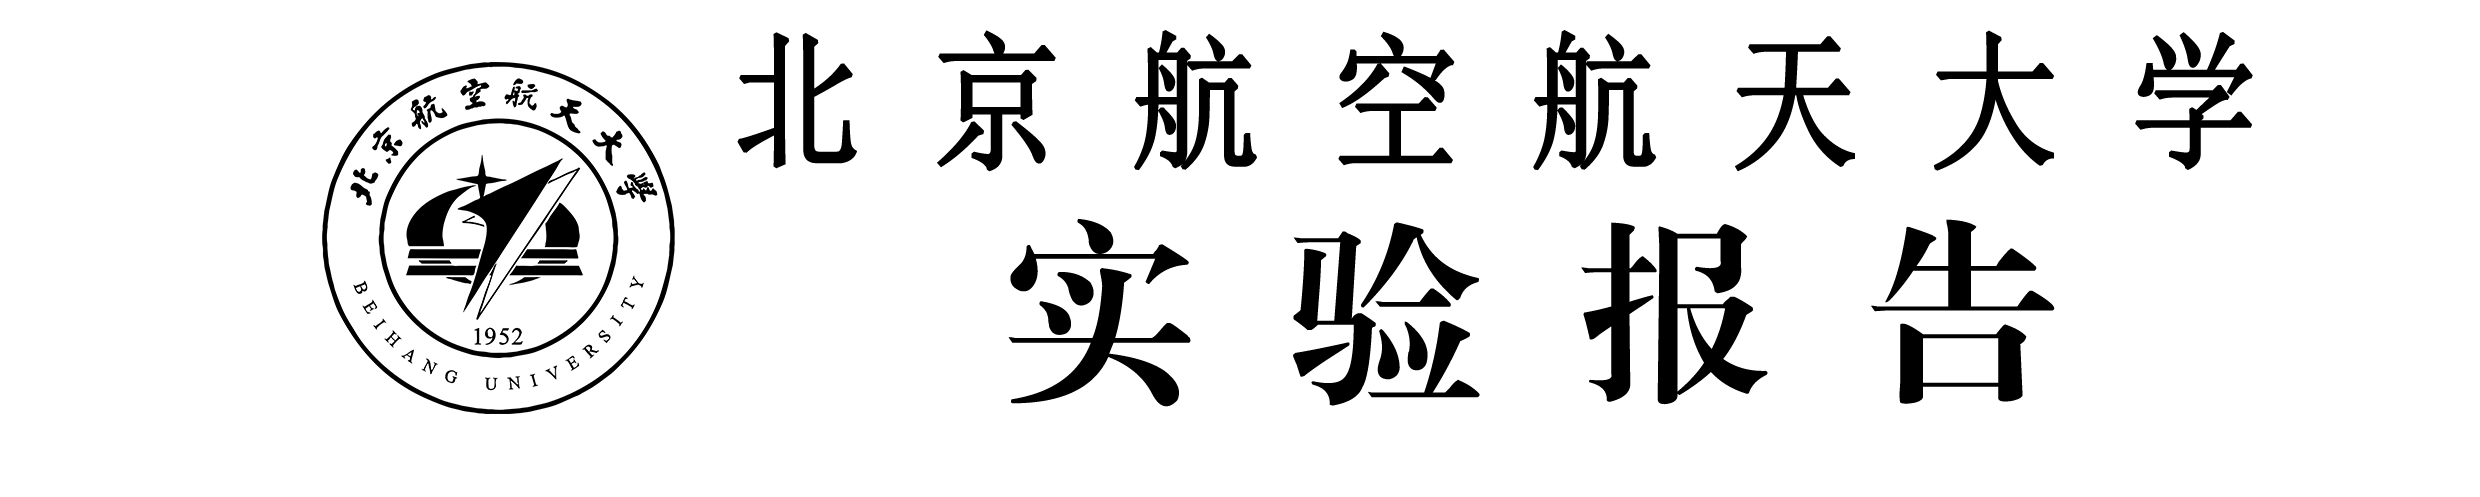
\includegraphics[width=13cm]{表头.png}
\end{figure}
\begin{center}
\textbf{{\large 实验名称:\uline{        弯曲法测横梁弹性模量       }}}
\end{center}

\section*{一、实验原理}
\subsection*{实验1.弯曲法测横梁弹性模量(弯曲仪法)}
将厚度为a,宽度为b的横梁放在相距为l的刀口上,在梁上两刀口的中点处挂一质量为m的砝码,这时梁被压弯,梁中心处下降的距离${\Delta}Z$称为松垂度。
在横梁发生微小弯曲时,梁的上半部发生压缩,下半部发生拉伸;而中间存在一个薄层,虽然弯曲但长度不变,称为中性面。

\begin{wrapfigure}{r}{0.4\textwidth}
  \vspace{-20pt}
  \begin{center}
    \includegraphics[width=0.48\textwidth]{弹性模量.jpg}
  \end{center}
  \vspace{-20pt}
  \vspace{-10pt}
\end{wrapfigure}

取中性面上相距为x、厚为dy、形变前长为dx的一段作为研究对象(如右图所示)。梁弯曲后所对应的张角为$d{\theta}$,长度改变量为$yd{\theta}$ ,所受拉力为$-dF$。根据胡克定律有
$$\displaystyle\frac{dF}{dS} = -E {\displaystyle\frac{yd{\theta}}{dx}}$$
式中dS表示形变层的横截面积,设横梁宽度为b,则$dS=b{\times}dy$ 。于是
$$dF = -Eb {\displaystyle\frac{d{\theta}}{dx} ydy}$$
此力对中性面的转矩dM为
 $$dM = {\mid}dF{\mid}y = Eb {\displaystyle\frac{d{\theta}}{dx}} y^2dy$$
积分得 
$$M = Eb {\displaystyle\frac{d{\theta}}{dx}} {\int_{\frac{-a}{2}}^{\frac{a}{2}}}y^2dy = {\displaystyle\frac{Eba^3}{12}} {\displaystyle\frac{d{\theta}}{dx}} (1)$$

如果将梁的中点O固定,在两侧各为$\displaystyle\frac{l}{2}$处分别施以向上的力$\displaystyle\frac{mg}{2}$ 。梁上距中点O为x,长为dx的一段,由于弯曲产生的下降$d({\Delta}Z)$为
 $$d({\Delta}Z)=({\displaystyle\frac{l}{2}}-x) d{\theta} (2)$$
当梁平衡时,由外力$\displaystyle\frac{1}{2}mg$对该处产生的力矩$\displaystyle\frac{1}{2}mg({\displaystyle\frac{l}{2}}-x)$等于由式 (1)求出的力矩M,即
$${\displaystyle\frac{1}{2}mg}({\displaystyle\frac{l}{2}}-x) = {\displaystyle\frac{Eba^3}{12}} {\displaystyle\frac{d{\theta}}{dx}}$$
 
从该式中解出$d{\theta}$代入式(2)中并积分,可求出驰垂度
 $${{\Delta}Z} = {\displaystyle\frac{6mg}{Ea^3b}}{\int_0^{\frac{l}{2}}({{\displaystyle\frac{l}{2}}-x)}^2dx} = {\displaystyle\frac{mgl^3}{4Ea^3b}}$$
于是弹性模量为
$$E = \displaystyle\frac{mgl^3}{4a^3b{\Delta}Z}$$

\subsection*{实验2.弯曲法测横梁弹性模量(霍尔传感器法)}
与前一实验同理,${\Delta}Z$属微小位移,用一般工具很难测准,在此可用霍尔位置传感器进行测量。将霍尔远见之于磁感应强度为B的磁场中,在垂直与磁场方向通以电流I,则与这二者相垂直的方向上将产生霍尔电势差:
 $$U_H =  kIB$$
式中k为元件的霍尔灵敏度。如果保持霍尔元件的电流I不变,而使其在一个均匀提督的磁场中移动,则输出的霍尔电势差变化量为
$${\Delta}U_H = kI{\displaystyle\frac{dB}{dZ}}{\Delta}Z = k{\Delta}Z$$ 
此式说明,若$\displaystyle\frac{dB}{dZ}$为常数,则${\Delta}U_H$与${\Delta}Z$成正比,其比例系数用K表示,称为霍尔传感器灵敏度。
\begin{figure}[htbp]
\centering
  \includegraphics[width=8cm]{均匀梯度.jpg}
\end{figure}
为实现均匀梯度的磁场,如图2所示,将两块相同的磁铁(磁铁截面积及表面磁感应强度相同)相对放置,即N极与N极相对,两磁铁之间留一定间隙,霍尔元件平行于磁铁放在该间隙的中轴上。间隙大小要根据测量范围和测量灵敏度要求而定,间隙越小,磁场梯度就越大,灵敏度就越高。磁铁街面要远大于霍尔元件,以尽可能减小边缘效应的影响,提高测量精度。
 
若磁铁间隙内中心截面处的磁感应强度为零,霍尔元件处于该处,则输出的霍尔电势差应该为零。当霍尔元件偏离中心沿Z轴发生位移时,由于磁感应强度不再为零,霍尔元件也就产生相应的电势差输出,其大小可以用数字电压表测量。由此可以将霍尔电势差为零时元件所处的位置作为位移参考点。

霍尔电势差与位移量之间存在一一对应的关系,当位移量较小(<2 mm)时,这一对应关系有良好的线性。
\section*{二、实验仪器}
${\romannumeral1}$.	霍尔位置传感器测杨氏模量装置一台(底座固定箱、读书显微镜、95型集成霍尔位置传感器、磁铁两块等);

${\romannumeral2}$.	霍尔位置传感器输出信号测量仪一台(包括直流数字电压表)。
\section*{三、实验步骤}
\subsection*{(1)调整系统}
\begin{enumerate}
\item 调节三维调节架的调节螺丝,使集成霍尔位置传感器探测元件处于磁铁中间的位置。
\item 用水准器观察是否在水平位置,若偏离时可以用底座螺丝调节。
\item 调节霍尔位置传感器的毫伏表。磁铁盒下的调节螺丝可以使磁铁上下移动,当毫伏表数值很小时,停止调节固定螺丝,最后调节调零电位器使毫伏表读数为零。
\item 调节读数显微镜,使眼镜观察十字线及分划板刻度线和数字清晰。然后移动读数显微镜前后距离,使能够清晰看到铜架上的基线。转动读数显微镜的鼓轮使刀口架的基线与读数显微镜内十字刻度线吻合,记下初始读数值。
\end{enumerate} 	
\subsection*{(2)测量数据 }
${\romannumeral1}$.逐次增加砝码 (每次增加10g砝码),相应从读数显微镜上读出梁的弯曲位移  及数字电压表相应的读数值 (单位mV)。以便于计算杨氏模量和霍尔位置传感器进行定标。(注意:在进行测量之前,要求符合上述安装要求,并且检查杠杆的水平、刀口的垂直、挂砝码的刀口处于梁中间,要防止外加风的影响,杠杆安放在磁铁的中间,注意不要与金属外壳接触,一切正常后加砝码,使梁弯曲产生位移  ;精确测量传感器信号输出端的数值与固定砝码架的位置Z的关系,也就是用读数显微镜对传感器输出量进行定标,检验  的关系 。)

${\romannumeral2}$.测量横梁两刀口间的长度d及测量不同位置横梁宽度b和梁厚度a。

${\romannumeral3}$.用逐差法按照公式进行计算,求得待测材料的杨氏模量,并估算不确定度,并把测量值与公认值进行比较。

${\romannumeral4}$.用一元线性回归法计算求出霍尔位置传感器的灵敏度 及其不确定度。
\subsection*{(3)数据处理}
${\romannumeral1}$.用一元线性回归计算霍尔位置传感器的灵敏度K及其不确定度。

${\romannumeral2}$.用逐差法计算待测材料的弹性模量E,并估算不确定度,计算与标准值的相对误差。
已知黄铜材料的标准值为$E_{Cu} = 10.55{\times
}10^10 N/{m^2}$,铸铁材料的标准值为$E_{Fe} = 18.15{\times
}10^10 N/{m^2}$。
\end{document}